\documentclass{ltjsarticle}

\usepackage{luatexja}
\usepackage{graphicx}
\usepackage[colorlinks=true,linkcolor=blue,citecolor=blue,urlcolor=blue]{hyperref}
\usepackage{xcolor}
\usepackage{mathtools}
\usepackage{siunitx}
\usepackage{amsmath}
\usepackage{amssymb}
\usepackage{sepnum} % sepnumパッケージを読み込む
\usepackage{at}
\usepackage{bm}
\usepackage{cancel}
\usepackage{titlesec}
\numberwithin{equation}{section} % 数式番号をセクションごとに分ける
\titleformat{\subsubsection}
  {\normalfont\large\bfseries}
  {\thesubsubsection}{1em}{}

\newcommand{\underlab}[3][.35ex]{%
  \mathrel{\mathop{#2}\limits_{\mathclap{\lower#1\hbox{\text{\footnotesize\textcircled{\scriptsize #3}}}}}}%
}



\usepackage[normalem]{ulem} % \uline, \uwave

% 直線 → \ulineunder、波線 → \uwaveunder
\newcommand{\ulineunder}[2]{%
  \underset{\smash{\text{\scriptsize #2}}}{\uline{\ensuremath{#1}}}%
}
\newcommand{\uwaveunder}[2]{%
  \underset{\smash{\text{\scriptsize #2}}}{\uwave{\ensuremath{#1}}}%
}

% 下線の“下げ量”と太さ(グローバル設定)
\setlength{\ULdepth}{1.2ex} 
\renewcommand\ULthickness{0.8pt} % 波線/直線の太さ


\usepackage[most]{tcolorbox}
\newtcolorbox{eqbox}[1]{%
  enhanced,
  colback=white, colframe=black,
  boxrule=0.4pt, arc=6pt,
  left=8pt, right=8pt, top=8pt, bottom=8pt, % 余白
  title={#1},                 % ← 引数がタイトルになる
  fonttitle=\bfseries,        % タイトルの体裁
  coltitle=black,
  colbacktitle=gray!10,       % タイトル帯の背景色(要らなければ white)
  attach boxed title to top left={yshift=-2mm, xshift=6pt}, % 箱内の左上に配置
  boxed title style={sharp corners, boxrule=0pt}, % タイトル枠線なし
}


\title{Introduction to Plasma Physics}
\author{中 陽太}
\date{2025年8月29日}

\begin{document}

\maketitle

% 目次
\tableofcontents

\section*{前書き}
 以下の内容は、主に

\cite{a} Francis F. Chen, "Introduction to Plasma Physics and Controlled Fusion"\par
\cite{b} 宮本健郎 『プラズマ物理の基礎』\par
\cite{c} EMANの物理学\\
を参照している。





\section{プラズマとは}
\subsection{自然界でのプラズマ}
 物質の温度を上げていくと、固体、液体、気体と相変化し、さらに温度を上げると、気体分子は原子から電子が剥ぎ取られ、プラスの電荷を持ったイオンと負の電荷を持った電子とが混じった気体になる。このような高温の電離ガス状態を\textcolor{red}{プラズマ}という。
固体、液体、気体と並んで、「第四の状態」と呼ばれることもある。

 一般的に、プラズマは真空中にしか存在しない。なぜなら、空気がプラズマを冷やし、イオンと電子を再び結合させるからである。自然界においては、宇宙空間は密度がかなり低いが一種のプラズマだし、
点灯中の蛍光灯の中やロウソクの炎などは全ての原子から電子が剥がれるほどではないがこれも一種のプラズマだし、さらにオーロラや電離層もプラズマだし、冬場に体験する静電気の放電や、溶接工事に使う電気放電、落雷などもプラズマである。太陽もまたプラズマの塊である。実に、この宇宙の99\%以上の場所がプラズマであって、地球のようなそうでない場所の方が珍しいくらいである。

 Saha方程式では、熱平衡状態にある気体において、イオン化の割合を教えてくれる。

\begin{eqbox}{Saha方程式}
\begin{equation}
\frac{n_i}{n_n} \approx 2.4 \times 10^{21} \frac{T^{3/2}}{n_i} e^{-U_i/KT} 
\end{equation}  
\end{eqbox}

ここで$n_i$はイオン化された原子の密度$[m^{-3}]$、$n_n$は原子の密度であり、$K$はボルツマン定数、$U_i$は気体のイオン化エネルギーである。

(1.1)式から、$T$が大きくなるにつれて$n_i$の割合が増える、つまり気体がプラズマ状態になることがいえる。これがプラズマが高温でのみ存在する理由である。

Saha方程式の物理的な意味を指摘すると、気体中の原子は熱エネルギーに分布があり、たまたま十分大きいエネルギーの衝突を受けると電子が飛び出して電離する。低温ではそのような“速い原子”は少なく、電離はまれ。Saha式の 
$\exp{(-U_i/KT)}$は「速い原子の数が温度に対して指数関数的に減る(=低温で急減)」ことを表す。また、いったん電離しても、電子と出会えば再結合して中性に戻る。つまり、再結合率は電子密度に依存する。これが$n_i ^{-1}$となる要因である。星間ガスでは 
$n_i \sim 1 cm^{-3}$と非常に低密度のため、再結合が遅く、高温でなくてもプラズマ状態が保たれやすい。


\subsection{プラズマの定義}
いかなるイオン化した気体をプラズマと呼ぶわけではない。プラズマの定義は次のように表される。
\begin{center}
プラズマとは、荷電粒子と中性粒子からなる準中性ガスであり、集団運動を示すものである。  
\end{center}

準中性ガスの説明は1.4節で説明する。集団運動について、これはプラズマ粒子間に働くクーロン力が遠距離まで作用することに起因している。クーロン力は$1/r^2$で減衰するのに対し、プラズマの場合、立体角を考慮すると、Aに対するBの体積は$r^3$に比例する。
そのため、遠距離においてもプラズマは影響し合っている。つまり、集団運動とは、局所的な条件だけでなく、遠隔領域におけるプラズマの状態にも依存する運動を指す。実際、これらの性質がプラズマ物理学という研究分野を豊かにしている。

\begin{figure}[htbp]
  \centering
  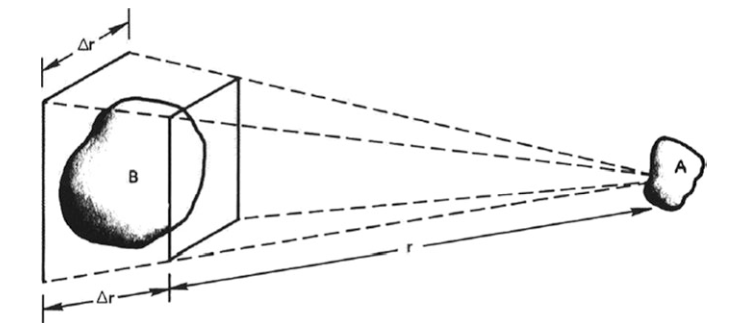
\includegraphics[width=0.7\linewidth]{solid_angle.png}
  \caption{遠距離に作用するクーロン力}
  \label{fig:sample}
\end{figure}


\subsection{温度の概念}
先に進む前に、温度の物理的な概念を見直そう。熱平衡状態の気体の速度分布はマクスウェル分布に従う。

\begin{eqbox}{一次元のマクスウェル分布}
\begin{equation}
f(u) = A \exp\left(-\frac{1}{2}mu^2/KT\right),\hspace{2pc} A = n\left(\frac{m}{2\pi KT}\right)^{1/2} \label{Max}
\end{equation}
\end{eqbox}

マクスウェル分布の導出は\url{https://www1.doshisha.ac.jp/~bukka/lecture/statistic/pdftext/std-02.pdf}を参照してほしい。

分布の幅は定数Tによって特徴づけられ、これを温度と呼ぶ。Tの正確な意味を理解するために、この分布における粒子の平均運動エネルギーを計算しよう。

\begin{equation}
 E_{av} = \frac{\int_{-\infty}^{\infty} \frac{1}{2}mu^2 f(u)du}{\int_{-\infty}^{\infty} f(u)du} \label{AV.K}
\end{equation}
ここで、
\begin{equation}
  v_{th} \coloneqq (2KT/m)^{1/2}, \hspace{1pc} y \coloneqq u/v_{th} \label{df.v_th}
\end{equation}
と定義すると、式\eqref{Max}は

\begin{center}
 $f(u) = A \exp(-u^2/v^2_{th})$ 
\end{center}
となり、式\eqref{AV.K}は

\begin{center}
  $E_{av} = \dfrac{\frac{1}{2}mAv^3_{th}\int_{-\infty}^{\infty}[\exp(-y^2)]y^2dy}{Av_{th}\int_{-\infty}^{\infty}[\exp(-y^2)]dy}$
\end{center}
となる。分子における積分部分について、部分積分を用いることで、

\begin{center}
  $\int_{-\infty}^{\infty} [-\frac{1}{2}\exp(-y^2)]'\cdot ydy = \left[-\frac{1}{2}\exp(-y^2)y\right]_{-\infty}^{\infty} - \int_{-\infty}^{\infty} -\frac{1}{2}\exp(-y^2)dy
  = \frac{1}{2}\int_{-\infty}^{\infty}\exp(-y^2)dy $
\end{center}
となり、積分部分が相殺される。これより、

\begin{equation}
  E_{av} = \frac{\frac{1}{2}mAv_{th}^3\frac{1}{2}}{Av_{th}} = \frac{1}{4}mv_{th}^2 = \frac{1}{2}KT \label{av.kenetic}
\end{equation}
が得られる。つまり、平均運動エネルギーは$\frac{1}{2}KT$である。

3次元への拡張は簡単であるため、導出を省き、結果を書くと、
\begin{equation}
  E_{av} = \frac{3}{2}KT
\end{equation}

上で見たように、$T$は$E_{av}$で記述できるため、プラズマ物理では温度をエネルギーの単位で表すことが慣習になっている。次元による混乱を避けるため$E_{av}$ではなく、$KT$で温度を表す。$KT = 1\space eV = 1.6 \time 10^{-19}\space J $から

\begin{center}
  $T= \dfrac{1.6\time 10{-19}}{1.38\time 10^{-23}} = {11,600}$
\end{center}
したがって、変換係数は、

\begin{equation}
  1\;\unit{eV}= {11,600}\; \unit{\kelvin}
\end{equation}
である。

面白いのは、プラズマは異なる温度を持つことである。電子とイオンは衝突頻度の違いにより、それぞれ異なる温度
  \( T_e, T_i \) を持つことがある。磁場中では、一種類の粒子でもローレンツ力の作用により、
  平行方向の温度 \( T_{\parallel} \) と垂直方向の温度 \( T_{\perp} \) が異なる場合がある。

次章に進む前に温度の概念の誤解を解かなければならない。高温であることが必ずしも「大量の熱」を意味するわけではないのだ。
例えば、蛍光灯内の電子温度は約 $2\times 10^4 \ \mathrm{K}$ だが、電子密度が低いため壁への熱伝達は小さい。
タバコの灰は高温でも、含まれる熱量が少ないため手に落ちても大きな火傷をしない。実験室プラズマでは $10^6 \ \mathrm{K}$ 程度の温度を持つこともあるが、
密度が $10^{18}$--$10^{19} \ \mathrm{m^{-3}}$ と低いため、壁加熱は深刻な問題とならない。


\subsection{デバイ遮蔽}
プラズマが示す特徴的な挙動は電位を遮蔽することである。図\refeq{fig.debye}のように電源に繋がれた2つの荷電粒子をプラズマ中に入れた状況を考える。それぞれの荷電粒子は逆符号の粒子を印加し、荷電粒子の周りにイオンまたは電子の「雲」が作られる。
荷電粒子のすぐ近くでは多くのイオン(電子)が引き寄せられるため、密度及びポテンシャルの勾配は高く、逆に遠方では低い。もしプラズマが低温で、熱運動がないのであれば、ポテンシャルは完全に遮蔽される。しかし、温度が高ければ、「雲」の
端では静電ポテンシャルが低いため、熱エネルギーがその壁を越えることができる。このときの「雲」の縁は、ポテンシャルエネルギーが粒子の熱エネルギーKTとほぼ等しくなる半径で生じ、遮蔽は完全ではない。
$KT/e$オーダーのポテンシャルがプラズマに漏れ込み、そこに有限の電場が存在することとなる。

\begin{figure}[htbp]
  \centering
  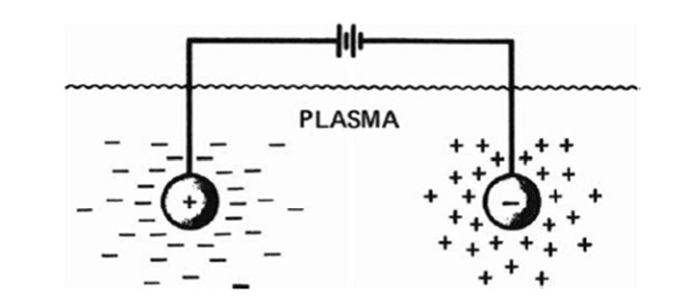
\includegraphics[width=0.7\linewidth]{debye.png}
  \caption{デバイ遮蔽の様子}
  \label{fig.debye}
\end{figure}


雲の中心(荷電粒子の位置)$x=0$のポテンシャルを$\phi _0$として、そこから減少し、無限遠で0になるポテンシャルを考える。このときの$\phi (x)$を求めてみよう。

一次元のポアソン方程式より、

\begin{equation}
  \epsilon_0 \nabla^2 \phi = \epsilon_0 \frac{d^2\phi}{dx^2} = -e(n_i - n_e) \hspace{1pc}  (Z=1) \label{poisson}
\end{equation}
\\
もし遠方の密度が$n_\infty$ であるなら、
\begin{center}
  $n_i = n_\infty$
\end{center}
となる。

ポテンシャルエネルギー$q\phi$の存在下において、電子の分布関数(ボルツマン分布)は、
\begin{equation}
  f(u) = A\exp[-\left(\frac{1}{2}mv^2 + q\phi\right)/KT_e]
\end{equation}
$q=-e$として、$u$で積分すると、

\begin{align}
  n_e &= \iiint A\exp[-\left(\frac{1}{2}mv^2 - e\phi\right)/KT_e]du^3 = \underline{A}e^{\frac{e\phi}{K T_e}} 
\underset{\equiv n_0}{\underline{\iiint e^{-\frac{m u^2}{2 K T_e}} \, du^3}}\\
       &= n_0 \exp(e\phi/KT_e)
\end{align}
遠方($x\to \infty$)で$\phi \to 0$より、
\begin{center}
  $n_e = n_0\cdot 1 = n_o = n_\infty$
\end{center}
これより、

\begin{center}
 $n_e =  n_\infty \exp(e\phi/KT_e)$
\end{center}
この式は3.5節でより物理的な洞察をもって導く。以上のことから、\eqref{poisson}式を書き直すと、

\[
\epsilon_0 \frac{d^2\phi}{dx^2}= en_\infty(e^{e\phi/KT_e} - 1)
\]
クーロンポテンシャルよりも運動エネルギーの方がはるかに大きい領域、つまり、$|e\phi / KT_e| \ll 1$の領域においてテーラー展開することで、
\[
 \epsilon_0 \frac{d^2\phi}{dx^2} = en_\infty\left[\frac{e\phi}{KT_e}+ \frac{1}{2}(\frac{e\phi}{KT_e})^2 + \cdots \right] \label{telor.1}
\]
となる。1次の項だけを考えると、

\begin{equation}
  \frac{d^2 \phi}{dx^2} = \frac{4\pi n_\infty e^2}{k_B T_e}\phi \label{debye.eq}
\end{equation}
を得る。ここでデバイ長を次のように定義する。

\begin{eqbox}{デバイ長}
\begin{equation}
 \lambda_D = \left(\dfrac{\epsilon_0 KT_e}{ne^2}\right)^{1/2} \label{debye}
\end{equation}
\end{eqbox}
これにより、式\eqref{debye.eq}の解は、
\begin{equation}
  \phi = \phi_0 \exp(-|x|/\lambda_D) \label{debye.poten}
\end{equation}
となる。\eqref{debye.poten}の表す意味は、試験電荷などといった外乱で生じた静電ポテンシャルが、距離とともに指数関数的に減衰し、その減衰の速さを決める長さが デバイ長 
$\lambda_D$\eqref{debye}ということである。具体的に、$1\lambda_D$離れると$\phi$は元の3\%、$3\lambda_D$で約5\%、$5\lambda_D$で1\%未満となる。それより十分大きなスケールではプラズマはほぼ中性に見える。
ゆえに、デバイ長は遮蔽の距離を決める尺度となる。

密度が増えると$\lambda_D$が減るのは、より電子が集まり、雲が濃くなるからである。$\lambda_D$の定義に使われているのは電子の温度である。なぜなら、電子はイオンに比べはるかに軽く、動きやすいため、電子が動くことにより遮蔽が生じるからである。

式\eqref{debye}の便利な式として、
\begin{align}
  \begin{split}
    \lambda_D &= 69(T_e/n)^{1/2}\si{\metre}, \hspace{2pc}  T_e \; \text{in} \; \si{\kelvin}\\
    \lambda_D &= 7430(KT_e/n)^{1/2}\si{\metre}, \hspace{2pc} KT_e \; \text{in} \; \si{\electronvolt}
  \end{split}
\end{align}
を与えておく。

ここまでで先に述べた「準中性」を定義できる。もし距離$L$の系が$\lambda_D$よりはるかに大きい場合、デバイ遮蔽が生じる。その外では$\nabla^2 \phi$は非常に小さく、$n_i$は$10^{-6}$以上の精度で$n_e$と等しい。
つまり、プラズマの「準中性」とは、$n$をプラズマ密度と呼ばれる一般的な密度とした場合、$n_i \simeq n_e \simeq n$とみなせるほど十分に中性であるが、興味深い電磁気力がすべて消滅するほど中性ではない状態のことである。 

デバイ遮蔽は、電子が非常に高速で互いに衝突せず、熱分布を維持できない場合に破られる。後述するように、電子が非常に高温の場合、電子衝突は稀である。この場合、イオンの正電荷に引き寄せられた一部の電子は、角度をつけて高速で進入し、惑星を周回する衛星のようにイオンの周囲を軌道運動する。
この仕組みは、後述するラングミュアプローブの解説で明らかになる。この効果を「反遮蔽」と呼ぶ者もいる。

1つの種類の系でもデバイ遮蔽は起きることがいえるが、ここでは立ち入らないことにする。

\subsection{プラズマパラメータ}
上で述べたように、デバイ遮蔽が生じるのは「雲」を作るのに十分な粒子が存在するときである。
\eqref{debye.poten}式からデバイ領域の粒子数$N_D$を計算できる。
\begin{equation}
  N_D = n\cdot \frac{4}{3}\pi \lambda_D ^3 = 1.38 \time 10^6T^{3/2}/n^{1/2} \hspace{1pc}(T\text{in}\, \si{\kelvin})
\end{equation}

「集団運動」をするためには、$\lambda_D \ll L$ に加えて、
\begin{equation}
  N_D \lll 1
\end{equation}
が必要である。この$N_D$を\textcolor{red}{プラズマパラメータ}と呼ぶ。

\subsection{プラズマの条件}
イオン化された気体がプラズマとみなされる条件は次の3つである。
\begin{enumerate}
  \item $\lambda_D \ll L$
  \item $N_D \ggg 1$
  \item $\omega \tau > 1$
\end{enumerate}
1,2の条件はこれまでに述べた。3について、プラズマ中の荷電粒子は、電磁力によって支配されている必要がある。
しかし、弱電離ガス(例:飛行機のジェット排気)では、中性粒子との衝突頻度が高すぎるため、運動は流体力学的な力に支配される。
典型的なプラズマ振動の角振動数を$\omega$、中性粒子との平均衝突時間を$\tau$とすると、プラズマと言えるためには、$\omega \tau > 1$が必要である。

\section{1粒子の運動}
\subsection{一様な電場と磁場}
プラズマの解析の難しい点は、流体のように個々の運動は考慮せず、集団運動で考える時もあれば、個々の粒子の集まりと考える時もあることである。
まずは簡単な例として、この章では、1粒子が電場または磁場においての運動を確認しよう。

\subsubsection{E=0}
この系では粒子は単にサイクロトロン運動をする。運動方程式は、
\begin{equation}
  m\frac{d\bm{v}}{dt} = q\bm{v}\times \bm{B} \label{E=0}
\end{equation}
ここで、$\bm{B}$はz方向を向き、$\bm{B}=B\bm{\hat{z}}$である。\eqref{E=0}式から、
\begin{equation}
\begin{gathered}
  m\dot{v}_x = qB v_y, \quad
  m\dot{v}_y = -qB v_x, \quad
  m\dot{v}_z = 0 \\
  \begin{aligned}
    \ddot{v}_x &= \frac{qB}{m}\dot{v}_y = -\left(\frac{qB}{m}\right)^2 v_x \\
    \ddot{v}_y &= -\frac{qB}{m}\dot{v}_x = -\left(\frac{qB}{m}\right)^2 v_y \label{E=0.eq}
  \end{aligned}
\end{gathered}
\end{equation} 
これは調和振動子を表し、その振動数を

\begin{eqbox}{サイクロトロン振動数}
\begin{equation}
  \omega_c = \frac{|q|B}{m} \label{cyclon}
\end{equation}
\end{eqbox}  
と定義すると、\eqref{E=0.eq}式の解は、

\[
v_{x,y} = v_\perp \exp(\pm i\omega_ct + i\delta_{x,y})
\]
ここで、\pm の符号はイオンであれば「+」、電子であれば「−」である。また、$v_\perp$は\bm{B}に垂直な速度の成分である。

位相の任意性から、
\begin{subequations}
  \begin{equation}
    v_x = v_\perp e^{i\omega_c t} = \dot{x} \label{normal.x}
  \end{equation}
と選ぶことにより、
  \begin{equation}
    v_y = \frac{m}{qB}\dot{v_x} = \pm \frac{1}{\omega_c}\dot{v_x} = \pm iv_\perp e^{i\omega_c t} = \dot{y} \label{normal.y}
  \end{equation}
\end{subequations}
これらを積分することで、

\begin{equation}
  x - x_0 = -i\frac{v_\perp}{\omega_c}e^{i\omega_c t}, \hspace{2pc} y -y_0 = \pm \frac{v_\perp}{\omega_c}e^{i\omega_c t} \label{larmor.eq}
\end{equation}
ここで、ラーモア半径を

\begin{eqbox}{ラーモア半径}
\begin{equation}
  r_L \equiv \frac{v_\perp}{\omega_c} = \frac{mv_\perp}{|q|B} \label{larmor.radi}
\end{equation}
\end{eqbox}  
を定義すると、\eqref{larmor.eq}式は、

\begin{equation}
  x - x_0 = r_L \sin \omega_c t, \hspace{2pc} y -y_0 = \pm r_L \cos \omega_c t
\end{equation}
となる。これは案内中心$(x_0, y_0)$を中心とした円軌道を表す。

粒子の回転運動の向きは磁場を減らそうとする向きであり、イオンと電子で反対になる。また、この働きからプラズマは反磁性であると言える。
粒子はこのサイクロトロン運動に加え、\bm{B}の方向に$v_z$で等加速度運動している。

\subsubsection{有限の電場}
次に、一様な電場がある場合を考える。同様に\bm{B}の方向にz軸をとり、$E_y=0$となるように\bm{E}をx-z面に配置するように座標空間をとる。
先の議論からz成分と他の成分は分けて考えることができる。運動方程式は、

\begin{equation}
  m\frac{d\bm{v}}{dt} = q(\bm{E} + \bm{v}\times \bm{B}) \label{finite.E}
\end{equation}
z成分は簡単に求まり、

\begin{equation}
  \frac{dv_z}{dt} = \frac{q}{m}E_z \hspace{3pc} \therefore v_z = \frac{qE_z}{m}t + v_{z0}
\end{equation}
となる。

残りの成分、つまり\bm{B}に垂直な面での運動は、\eqref{finite.E}式から
\begin{align}
  \begin{split}
    \frac{dv_x}{dt} &= \frac{q}{m}E_x \pm \omega_c v_y\\
    \frac{dv_y}{dt} &= 0 \mp \omega_c v_x
  \end{split}
\end{align}
微分してそれぞれ計算すると、

\begin{subequations}
  \begin{align}
    \ddot{v_x} &= -\omega_c^2v_x\\
    \ddot{v_y} &= \mp \omega\left(\frac{q}{m}E_x \pm \omega_c v_y\right) = -\omega_c\left(\frac{E_x}{B}+v_y\right) \label{v_e.eq}
  \end{align}
\end{subequations}
  ここで、前節との類似点から粒子がサイクロトロン運動をすることを見越して、

\begin{equation}
  v_y = \uwaveunder{\pm v_\perp e^{i\omega_c t}}{サイクロトロン運動}+v_E \label{if.ve}
\end{equation}
を仮定する\footnote{Introduction to Plasma Physics and Controlled Fusionの方法ではなく、\url{https://youtu.be/6PL0fKNmRmQ}での方法に従った。}。これの2階微分は、

\begin{equation}
  \begin{aligned}
    \ddot{v_y} = \mp i\omega_c ^2 v_\perp e^{i\omega_c t} &= -\omega_c ^2 (\ulineunder{\pm iv_\perp e^{i\omega_c t}+v_E}{$=\,v_y$})+\omega_c ^2 v_E\\
                                                          &= -\omega_c ^2(-v_E + v_y)
  \end{aligned}
\end{equation}
これと\eqref{v_e.eq}式を比較すると、

\begin{equation}
  v_E = -\frac{E_x}{B}
\end{equation}
となる。これより、\eqref{if.ve}式を書き直すと
\begin{equation}
  v_y = \pm iv_\perp e^{i\omega_c t} - \frac{E_x}{B}
\end{equation}
さらに、
\begin{equation}
  v_x = \mp \frac{1}{\omega_c}\dot{v_y} = v_\perp e^{i\omega_c t}
\end{equation}
となる。サイクロトロン運動は以前と同様であるが、案内中心のy方向へのドリフト$v_E$が重ね合わされる。
$v_E$の一般式は、ベクトル形式で表すことができる。

\[
  \bm{E} \times \bm{B} = 
\begin{pmatrix}
E_x \\ 0 \\ E_z
\end{pmatrix}
\times
\begin{pmatrix}
0 \\ 0 \\ B
\end{pmatrix}
=
\begin{pmatrix}
0 \\ -BE_x \\ 0
\end{pmatrix}
\]
となることから、

\begin{equation}
  \boxed{\bm{v}_E = \frac{\bm{E}\times \bm{B}}{B^2}} \label{general.ve}
\end{equation}
と表せる。この$\bm{v}_E$は\textcolor{red}{$\bm{E}\times \bm{B}$ドリフト}と呼ばれる。$v_E$は$q$,$m$,$v_\perp$に依存しない。

このドリフトが生じる背景は図\refeq{fig.EB_drift}を見てほしい。まず半回転する間において、粒子は電場$E_x$により加速され、$r_L$が大きくなる。反対に、もう半回転する間は$r_L$は小さくなる。
この差が$-y$方向へのドリフトを生じさせる。イオンと電子では、$\bm{E}\times \bm{B}$ドリフトは同じ方向であるが回転は逆となる。

\begin{figure}[htbp]
  \centering
  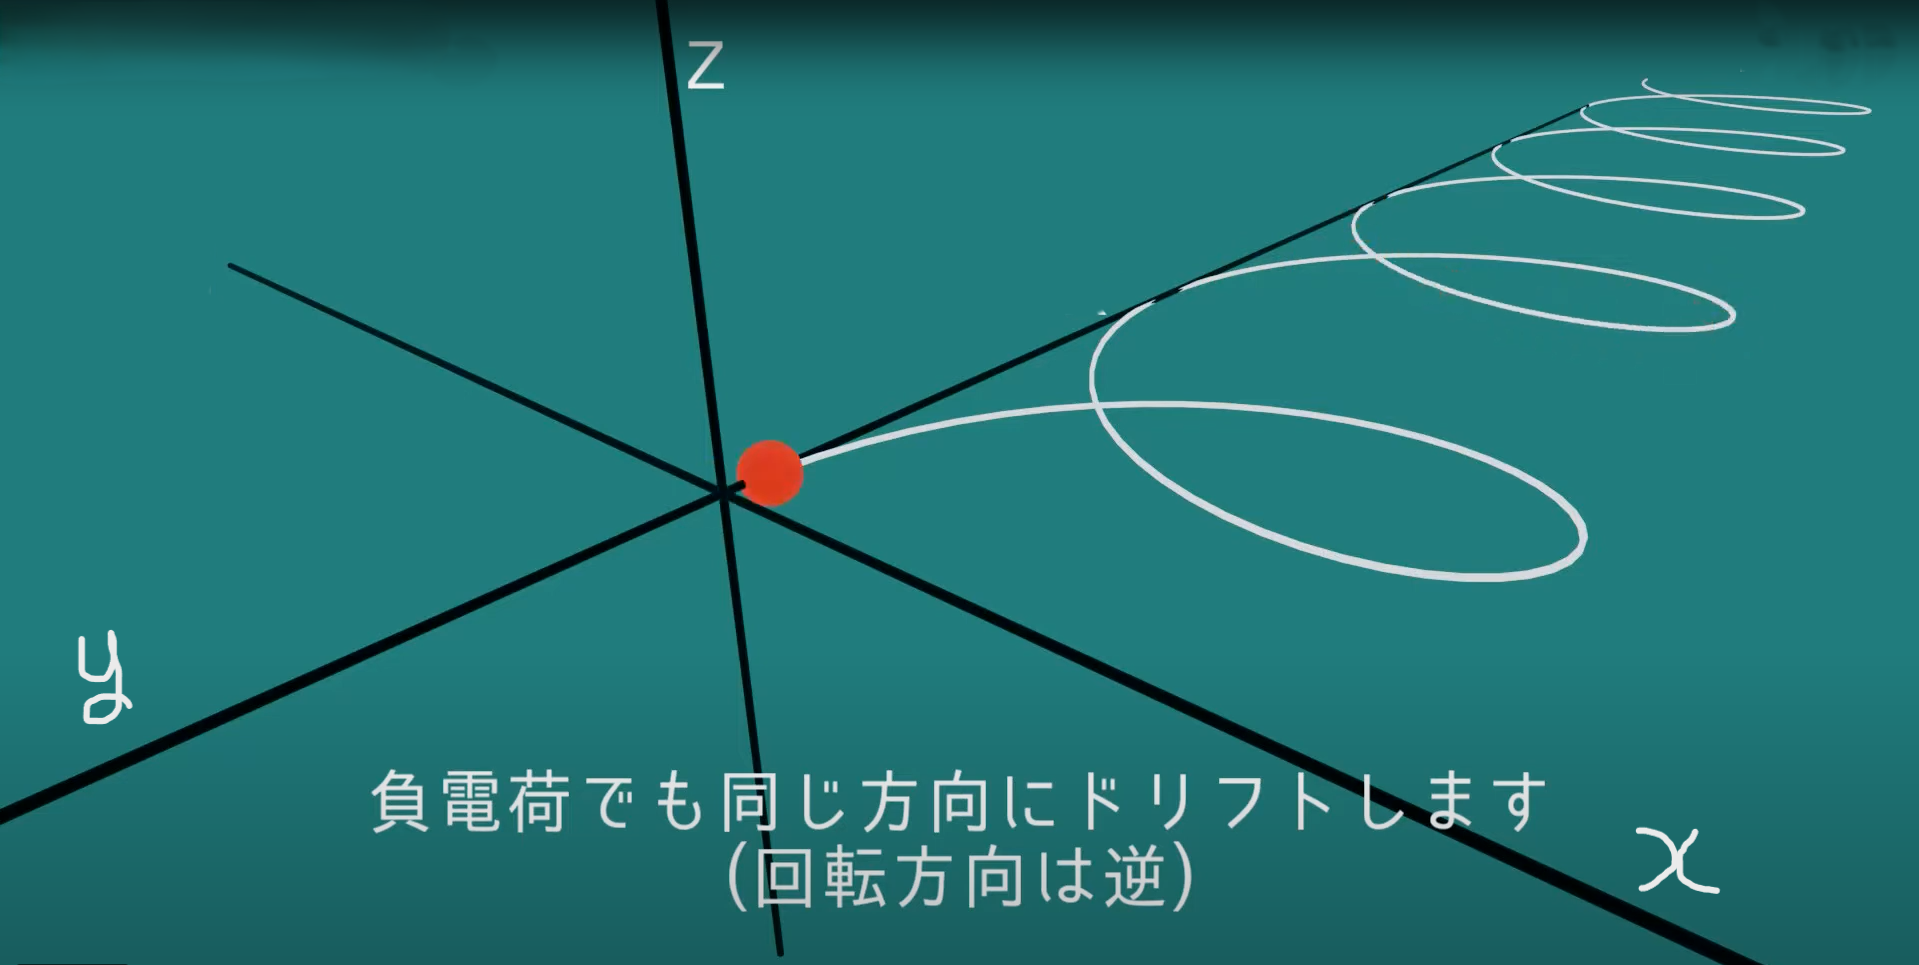
\includegraphics[width=0.7\linewidth]{EB_drift.png}
  \caption{\bm{E}\times \bm{B}ドリフト\,+\,サイクロトロン運動の軌道}
  \label{fig.EB_drift}
\end{figure}

これらを踏まえて、z方向を含めた粒子の運動は、
\[
\bm{v} =
\left(
  \vcenter{\hbox{\shortstack{磁場に平行なクーロン力による\\等加速度直線運動}}}
\right)
+ \left(\text{サイクロトロン運動}\right)
+ \left(\text{\( \bm{E}\times\bm{B} \) ドリフト}\right)
\]
となる。もし$\bm{B}\perp \bm{E}$であるならば、第一項の運動はなくなる。

\subsubsection{重力場}
先の結果は$q\bm{E} \to \bm{F}$と置き換えることで一般的な力$\bm{F}$に適用できる。$\bm{F}$による案内中心のドリフトは\eqref{general.ve}式より

\begin{equation}
  \boxed{\bm{v}_f = \frac{1}{q}\frac{\bm{F}\times \bm{B}}{B^2}} \label{drift_F}
\end{equation}
特に、$\bm{F}$が重力$m\bm{g}$であるとき、

\begin{equation}
  \boxed{\bm{v}_g = \frac{m}{q}\frac{\bm{g}\times \bm{B}}{B^2}}
\end{equation}
となる。ここで注意すべきは、$\bm{v_E}$では粒子によらず同じ方向であったが、$\bm{v_g}$ではイオンと電子で方向が逆になる。
プラズマ中で電子とイオンが逆向きに動くことは電流を流れることを意味する。電子だけ動いても電流が流れると思うかもしれないが、
プラズマでは荷電分離がすぐに電場を生んで打ち消してしまうので、持続的に電流が流れるためには電子とイオンが逆向きに動く必要がある。
この$\bm{v}_g$により生じる電流密度は、

\begin{equation}
  \bm{j} = nev_{g,i} + n\cdot (-e)v_{g,e} = n(M+n)\frac{\bm{g}\times \bm{B}}{B^2}
\end{equation}
となる。

実際には、地上の重力$\bm{g}$は小さいため、$|\bm{v}_g|$は通常、無視してよい。しかし、磁力線が曲がっている場合、後述するように、遠心力に起因する「有効重力」が生じる。
遠心力は「重力」不安定と呼ばれるプラズマ不安定性の基盤であり、これは実際の重力とは無関係である。

\subsection{非一様磁場}
これまで見てきたように、一様な場では厳密な解を求めることができた。しかし、空間や時間によって変わる電場や磁場下での粒子の運動は非常に複雑であり、厳密解が得ることは難しい。
そこで近似解を求める方法として、非一様性を表すスケール長$L$を用いて、微小量$r_L/L$で展開することがよくなされる。この種の理論は「軌道理論」と呼ばれ、非常に複雑である。
ここでは、同時には1つの非一様性しか含まないような最も簡単な場合について考える。

\subsubsection{\nabla \bm{B} \perp \bm{B} : grad Bドリフト}
図\refeq{fig.gradB_drift}のようにz方向の磁場がy方向に応じて密度(大きさ)が増えるとする。
この場合の粒子の軌道は予想できる。上部と下部での磁場の大きさの違いによりラーモア半径が変わり、その差がドリフトを生み出す。($\bm{E}\times \bm{B}$ドリフトと同じ原理。)

1回転について平均したローレンツ力 $\bm{F} = q\bm{v} \times \bm{B}$について考える。$\bar{F_x}$について、図\refeq{fig.gradB_drift}からわかるように、下部および上部での回転それぞれで$F_x$はちょうど打ち消し合うため、$\bar{F_x}=0$である。

\begin{figure}[htbp]
  \centering
  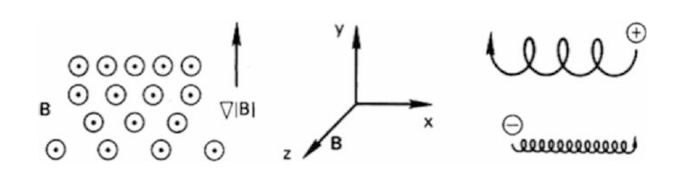
\includegraphics[width=0.7\linewidth]{gradB_drift.png}
  \caption{非一様磁場でのドリフト}
  \label{fig.gradB_drift}
\end{figure}

$\bar{F_y}$は近似的に求めることになるが、ゆがみのない粒子軌道を考えることから出発する。ゆがみのない粒子軌道は、一様磁場で\eqref{normal.x},\eqref{normal.y},\eqref{larmor.eq}式とすでに求めた。
$r_L/L\ll 1$を満たす任意の場所において$\bm{B}$は1次までのテーラー展開で表せる。(2次以上は無視できるため。)

\begin{equation}
  \bm{B} = \bm{B}_0 + (\bm{r}\cdot \nabla)\bm{B} + \cdots
\end{equation}
\[
  B_z = B_0 + y(\partial B_z/\partial y) + \cdots
\]
展開点に$x_0=0, y_0=0$を選び、\eqref{normal.x}式で実部を取ると、

\begin{equation}
  F_y = -qv_x B_z(y) = -qv_\perp (\cos{\omega_ct})\left[B_0 \pm r_L(\cos{\omega_c t})\frac{\partial B}{\partial y}\right] \label{grad_B_drift}
\end{equation}
\eqref{grad_B_drift}式の第一項は1回転で平均すれば0となる。第二項は$\cos^2{\omega_c t}$の平均が1/2であることから、

\begin{equation}
  \bar{F_y} = \mp q v_\perp r_L \frac{1}{2}\frac{\partial B}{\partial y}
\end{equation}
これより、案内中心のドリフト速度は\eqref{drift_F}式より、

\begin{equation}
  \bm{v}_{gc} = \frac{1}{q}\frac{\bm{F} \times \bm{B}}{B^2} = \frac{1}{q} \frac{\bar{F_y}}{|B|}\hat{\bm{x}} = \mp \frac{v_\perp r_L}{B} \frac{1}{2} \frac{\partial B}{\partial y}\hat{\bm{x}}
\end{equation}
これには平均化した力をそのまま\eqref{drift_F}式に使っていいのかといった疑問を抱くかもしれないが、grad B ドリフトよりも旋回運動の方がずっと速いため、平均を考えた1周はドリフトにとっては一瞬であると考えられるので問題はない。
これをより一般的に書くと、$\bm{E}\times \bm{B}$ドリフトと同じ計算で、

\begin{equation}
  \boxed{\bm{v}_{\nabla B} = \pm \frac{1}{2}v_\perp r_L \frac{\bm{B}\times \nabla B}{B^2}} \label{df.grad_B_drift}
\end{equation}

この$\bm{v}_{\nabla B}$は\textcolor{red}{grad B ドリフト}と呼ばれる。$\pm$が表すようにイオンと電子で方向が反対になり、$\bm{B}$に垂直な方向に電流が生じる。
$\bm{v}_{\nabla B}$の正確な計算には、平均化プロセスにおいてドリフトを含む正確な軌道の使用が必要となる。

\subsubsection{湾曲磁場:曲率ドリフト}
磁力線が一定の曲率半径$R_c$で湾曲しており、|B|は一定である場合を考える(図\refeq{fig.curvature})。
粒子が熱運動で磁力線に沿って移動する際に、粒子が受ける遠心力により案内中心のドリフトが起きる。ランダムな速度の$\bm{B}$方向の2乗平均を$v_\parallel ^2$と表すと、
平均的な遠心力は

\begin{equation}
  \bm{F}_{cf} = \frac{mv_\parallel ^2}{R_c} \hat{\bm{r}} = mv_\parallel ^2 \frac{\bm{R}_c}{R_c ^2}
\end{equation}
これによって起きるドリフト速度は\eqref{drift_F}式より、

\begin{equation}
  \boxed{\bm{v}_R = \frac{1}{q}\frac{\bm{F}_{cf} \times \bm{B}}{B^2} = \frac{mv_\parallel ^2 }{qB^2} \frac{\bm{R}_c \times \bm{B}}{R_c ^2}}
\end{equation}
このドリフト$\bm{v}_R$は\textcolor{red}{曲率ドリフト}と呼ばれる。

\begin{figure}[htbp]
  \centering
  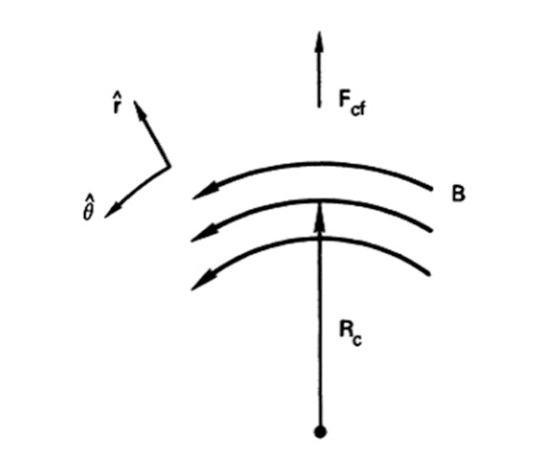
\includegraphics[width=0.7\linewidth]{curvature.png}
  \caption{湾曲磁場}
  \label{fig.curvature}
\end{figure}

湾曲磁場では、曲率ドリフトに加えてgrad B ドリフトも生じる。次にgrad B ドリフトを曲率半径方向の|B|の減少を考慮して計算してみよう。真空中ではマクスウェル方程式より、$\nabla \times \bm{B} = 0$が成り立っている。
図\refeq{fig.curvature} の円柱座標において、$\bm{B}$は$\theta$方向の成分のみ、$\nabla B$はr方向の成分のみであるため、$\nabla \times \bm{B}$はz成分のみとなる。
円柱座標系で表されたベクトル場$\bm{A}$の回転$\nabla \times \bm{A}$は、
\[
 \nabla \times \bm{A} = \left\{\frac{1}{r}\frac{\partial A_z}{\partial \theta}\right\}\bm{e}_r + \left\{\frac{\partial A_r}{\partial z}-\frac{\partial E_z}{\partial r}\right\}\bm{e}_\theta + \dfrac{1}{r}\left\{\frac{\partial}{\partial r}(rA_\theta) - \frac{\partial E_r}{\partial \theta}\right\}\bm{e}_z
\]
で表されるので、

\begin{equation}
  (\nabla \times \bm{B})_z = \frac{1}{r}\frac{\partial}{\partial r} (rB_\theta) = 0 \hspace{2pc} B_\theta \propto \frac{1}{r} \hspace{2pc} \therefore |B| \propto \frac{1}{R_c}
\end{equation}
また、
\[
  \nabla |B| = \frac{d|B|}{dr}\hat{r} \propto -\frac{1}{r^2}\hat{r} 
\]
より、
\begin{equation}
  \frac{\nabla |B|}{|B|} = -\frac{\bm{R}_c}{R_c ^2}
\end{equation}
これより、\eqref{df.grad_B_drift}式を用いて、

\begin{equation}
  \bm{v}_{\nabla B} = \mp \frac{1}{2}\frac{v_\perp r_L}{B^2}\bm{B}\times |B| \frac{\bm{R}_c}{R_c ^2} = \pm \frac{1}{2} \frac{v_\perp ^2}{\omega_c}\frac{\bm{R}_c \times \bm{B}}{R_c ^2B^2} = \frac{1}{2}\frac{m}{q}v_\perp ^2 \frac{\bm{R}_c \times \bm{B}}{R_c ^2 B^2}
\end{equation}

前の$\bm{v}_R$にこれを加えて、真空湾曲磁場中でのドリフトは
\begin{equation}
  \boxed{\bm{v}_R + \bm{v}_{\nabla B} = \frac{m}{q} \frac{\bm{R}_c \times \bm{B}}{R_c ^2 B^2}\left(v_\parallel ^2 + \frac{1}{2}v_\perp ^2\right)}
\end{equation}
となる。

このようなドリフトが加わるのは望ましくない。なぜなら、曲率ドリフト$\bm{v}_R$とgrad B ドリフト$\bm{v}_{\nabla B}$が 同じ垂直方向(イオンの場合、図\refeq{fig.curvature}では上向き)に出て加算されるため、案内中心は一方向に単調にずれていき、
最終的に外に出てしまう。核融合プラズマを閉じ込める目的で磁場をトーラス状にしても閉じ込められないのである。

 マクスウェル分布の場合、\eqref{av.kenetic}から、$v_\perp$が2自由度を含むことに注意すると、$\bar{v_\parallel ^2}$、$\frac{1}{2}\bar{v_\perp ^2}$は
 \begin{align*}
  \frac{1}{2}m\bar{v_\parallel ^2} &= \frac{1}{2}KT \hspace{2pc} \bar{v_\parallel ^2} = \frac{KT}{m}\\
  \frac{1}{2}m\bar{v_\perp ^2} &= KT \hspace{2pc} \frac{1}{2}\bar{v_\perp ^2} = \frac{KT}{m}
 \end{align*}
と表される。\eqref{df.v_th}を用いることで、平均曲率場ドリフトを次のように記述できる。

\addtocounter{equation}{-1}% 親番号を 2.30 に合わせる
\begin{subequations}
  \begin{equation}\label{eq:230a}
    \bar{\bm{v}}_{R+\nabla B} = \pm \frac{v_{th}^2}{R_c \omega_c}\hat{\bm{y}} = \pm \frac{\bar{r_L}}{R_c}v_{th} \bar{\bm{y}}
  \end{equation}
\end{subequations}
ここで、$\bar{\bm{y}}$は$\bm{R}_c \times \bm{B}$の向きである。この式から$\bar{\bm{v}}_{R+\nabla B}$は粒子の電荷には依存するが、質量には依存しないことがいえる。

\subsubsection{$\nabla B \parallel \bm{B}$ : 磁気ミラー}
磁場のだいたいの方向がz方向で、z方向に強さの変化する磁場を考える。磁場は軸対称であるとすると、$B_\theta = 0$、$\partial/\partial \theta = 0$である。(図\refeq{fig.mirror})
このような磁場が粒子を捕捉できるような力を生み出すことを以下に示そう。

\begin{figure}[htbp]
  \centering
  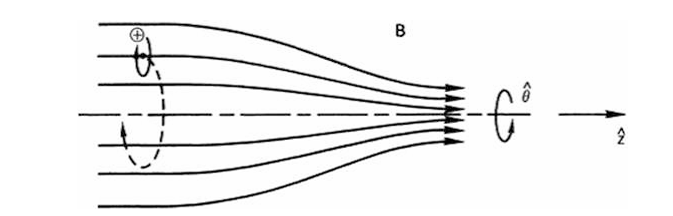
\includegraphics[width=0.7\linewidth]{magnetic_mirror.png}
  \caption{ミラー磁場中での粒子のドリフト}
  \label{fig.mirror}
\end{figure}

$\nabla \cdot \bm{B} = 0$より、

\begin{equation}
  \frac{1}{r}\frac{\partial}{\partial r}(rB_r) + \frac{\partial B_z}{\partial z} = 0
\end{equation}
ここで、円柱座標系で表されたベクトル場$\bm{A}$の発散が
\[
  \nabla \cdot \bm{A} = \frac{1}{r}\frac{\partial}{\partial r}(rA_r) + \frac{1}{r}\frac{\partial A_\theta}{\partial \theta} + \frac{\partial A_z}{\partial z}
\]
で表せることを用いた。
$\frac{\partial B_z}{\partial z}$の値が$r=0$で与えられ、$r$とともにあまり大きく変化しないとすると、近似的に、

\begin{equation}
  \begin{gathered}
    rB_r = -\int_{0}^{r} r\frac{\partial B_z}{\partial z}dr \simeq -\frac{1}{2}r^2\left[\frac{\partial B_z}{\partial z}\right]_{r=0}\\
    B_r = -\frac{1}{2}r\left[\frac{\partial B_z}{\partial z}\right]_{r=0}    
  \end{gathered} \label{term1234}
\end{equation}
となる。$r$による$|\bm{B}|$の変化はgrad B ドリフトを引き起こすが、$\partial B/\partial \theta = 0$なので、$\nabla B$に$\theta$方向の成分は存在しない。よって、$\bm{B}\times \nabla B$のr方向成分は0であるから、半径方向にはgrad B ドリフトは存在しない。
ローレンツ力の成分は

\begin{align}
  \begin{split}
    F_r     &= q(\underlab{v_\theta B_z}{1}-v_z \cancel{B_\theta})\\
    F_\theta&= q(\underlab{-v_r B_z}{2}+\underlab{v_z B_r}{3})\\
    F_z     &= q(v_r \cancel{B_\theta}-\underlab{v_\theta B_r}{4})
  \end{split}
\end{align}

$B_\theta = 0$より2つの項が消える。➀項と➁項は通常のラーモア運動を引き起こす項である。➂項は軸上では消え、軸から離れたところでは、

\[
  \bm{F} \times \bm{B} = (F_\theta \hat{\theta}) \times (B_r \hat{r}+B_z \hat{z}) = F_\theta B_z \hat{r} - F_\theta B_r \hat{z}
\]
ここで、$B_z \gg B_r$の近似を用いると、
\[
 \bm{F} \times \bm{B} = F_\theta B_z \hat{r} = qv_zB_rB_z\hat{r}
\]
これをドリフトの一般式に代入すると、
\begin{equation}
  \bm{v}_{d} = \frac{\bm{F} \times \bm{B}}{qB^2} = \frac{qv_zB_rB_z}{q(B_z^2+B_r^2)}\hat{r} \simeq v_z \frac{B_r}{B_z}\hat{r} \hspace{2pc} (B_z \gg B_r) \label{v_d,r}
\end{equation}
となり、r方向のドリフトを引き起こすことがわかる。

次に、磁力線の幾何から磁力線に沿う運動の必要条件を求めてみる。磁力線に沿った弧長の微小距離を$ds$とすると、$ds$は$\bm{B}$に平行なので、

\[
 \frac{dr}{ds} = \frac{B_r}{B}, \qquad \frac{dz}{ds} = \frac{B_z}{B} \hspace{1pc} \to \hspace{1pc} \frac{dr}{dz} = \frac{B_r}{B_z} 
\]
が成り立つ。これより$r$の変化率は、
\begin{equation}
  \frac{dr}{dt} = \frac{dr}{dz}\frac{dz}{dt} = \frac{B_r}{B_z}v_z \label{r_rate}
\end{equation}
となる。\eqref{v_d,r}式と\eqref{r_rate}式を比較すると完全に一致していることがわかる。つまり、ドリフト運動で動くr方向の速度と磁力線のr方向の変化率は一致する。
これはドリフト運動が磁力線に沿って移動していることを表す。長くなったが、以上をまとめると、➂項の力が$r$方向のドリフトを引き起こすが、このドリフトは単に案内中心を磁力線に沿わせるように働く。

結局、注目すべきは➃項である。\eqref{term1234}式より、

\begin{equation}
  F_z = \frac{1}{2}qv_\theta r(\partial B_z/\partial z)
\end{equation}
となる。1周にわたって平均をとるが、簡単のため、案内中心が軸上にあるような粒子を考える。このとき、$v_\theta$は回転の間、一定であり、qが+のときは時計回り、-のときは反時計回りであることを考えると、
$v_\theta$は$\mp v_\perp$と書ける。$r=r_L$から、平均的な力は

\begin{equation}
  \bar{F_z} = \mp \frac{1}{2}qv_\perp r_L\frac{\partial B_z}{\partial z} = \mp \frac{1}{2}q\frac{v_perp ^2}{\omega_c}\frac{\partial B_z}{\partial z} = -\frac{1}{2}\frac{mv_\perp ^2}{B}\frac{\partial B_z}{\partial z}
\end{equation}
となる。
回転粒子の磁気モーメントを
\begin{eqbox}{磁気モーメント}
\begin{equation}
 \mu \equiv \dfrac{\frac{1}{2}mv_\perp ^2 }{B}  \label{df.mag_moment}
\end{equation}
\end{eqbox}
で定義すると

\begin{equation}
  \bar{F_z} = -\mu (\partial B_z / \partial z)
\end{equation}
となる。一般的には、

\begin{equation}
  \bm{F}_\parallel = -\mu (\partial B /\partial s) = -\mu \nabla_\parallel B \label{F.mag_moment}
\end{equation}
と書かれる。\eqref{df.mag_moment}式の定義が、面積$A$、電流$I$の円電流に関する磁気モーメントの定義$\mu= IA$と等価であることに注目してほしい。
1価に帯電したイオンの場合、電荷$e$が1秒間に$\omega_c/2\pi$回回転することにより電流$I$が発生する。$I=e\omega_c/2\pi$、$A=\pi r_L ^2 = \pi v_\perp ^2/\omega_c ^2$より

\[
 \mu = \frac{\pi v_\perp ^2}{\omega_c ^2}\frac{e\omega_c}{2\pi} = \frac{1}{2}\frac{mv_\perp ^2}{B}
\]
となる。

$\mu$が不変量であることを証明しよう。運動方程式の$\bm{B}$に沿った成分は\eqref{F.mag_moment}式を用いて

\begin{equation}
  m\frac{dv_\parallel}{dt} = -\mu \frac{\partial B}{\partial s}
\end{equation}
左辺に$v_\parallel$を、右辺にそれと同値の$ds/dt$をかけると、

\begin{equation}
  mv_\parallel \frac{dv_\parallel}{dt} = \frac{d}{dt}\left(\frac{1}{2}mv_\parallel ^2\right) = -\mu \frac{\partial B}{\partial s}\frac{ds}{dt} = -\mu \frac{dB}{dt} \label{time_shift_B}
\end{equation}
ここで、$dB/dt$は粒子から見た$B$の変化であり、$B$自身は時間に対して変化していない。粒子のエネルギーは保存しているはずだから、

\begin{equation}
  \frac{d}{dt}\left(\frac{1}{2}mv_\parallel ^2 + \frac{1}{2}mv_\perp ^2\right) = \frac{d}{dt}\left(\frac{1}{2}mv_\parallel ^2 + \mu B\right) = 0
\end{equation}
他にローレンツ力も働いているが仕事をしないので、考えるエネルギーは運動エネルギーのみで良い。\eqref{time_shift_B}式から

\[
 -\mu \frac{dB}{dt} + \frac{d}{dt}(\mu B) = 0
\]
したがって、
\begin{equation}
  d\mu/dt = 0
\end{equation}
が証明できた。

$\mu$の不変性は、初期のプラズマ閉じ込め計画の1つであった「磁気ミラー」の基礎である。熱運動によって粒子が弱磁場から強磁場へ動いたとき、$B$が増えるため、$\mu$を一定に保つために$v_\perp$も増える。
全運動エネルギーは一定なので、このとき必然的に$v_\parallel$は減少する。もし$B$がミラーの「のど」の部分で十分に強ければ、$v_\parallel$は最終的に0となり、弱磁場の方へ反射される。

このような状況は2つのコイルさえあれば実現できる(図\refeq{fig.trap})。2つのコイルによってできる非一様磁場は2つの磁気ミラーを形成し、その間にプラズマを閉じ込めることができる。この効果はイオンにも電子にも働く。

\begin{figure}[htbp]
  \centering
  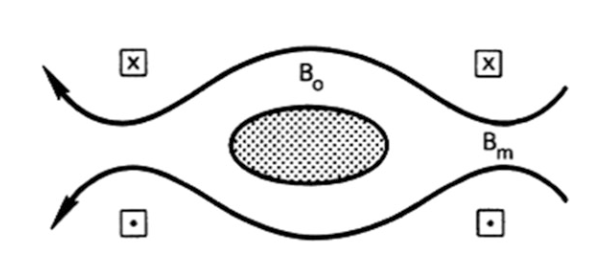
\includegraphics[width=0.7\linewidth]{trapped.png}
  \caption{磁気ミラー間に閉じ込められたプラズマ}
  \label{fig.trap}
\end{figure}

しかし、この閉じ込めは完璧ではない。例えば、$v_\perp=0$の粒子は磁気モーメントを持たず、$\bm{B}$に沿った力を感じない。また、もし最大磁場である$B_m$が十分に大きくなかった場合、$v_\parallel$が0にならず、そのまま通過していくこともあるだろう。
では、どのような$B_0$ないしは$B_m$であれば粒子は逃げていってしまうのであろうか?中央の面での粒子の速度を$v_{\perp 0}$、$v_{\parallel 0}$、反射点での速度を$v_\perp ^\prime$、($v_\parallel =0$)とする。
さらに反射点での磁場を$B^\prime$とすると、$\mu$の不変性により

\begin{equation}
  \frac{1}{2}mv_{\perp 0} ^2 /B_0 = \frac{1}{2}mv_\perp ^{\prime 2}/B^\prime \label{mu.eq}
\end{equation}
また、エネルギー保存則から、

\begin{equation}
  v_\perp ^{\prime 2} = v_{\perp 0}^2 + v_{\parallel 0}^2 \equiv v_0 ^2 \label{v_parallel.eq}
\end{equation}
が成り立っている。\eqref{mu.eq}、\eqref{v_parallel.eq}式から、

\begin{equation}
  \frac{B_0}{B^\prime} = \frac{v_{\perp 0 ^2}}{v_\perp ^\prime 2} = \frac{v_{\perp0}^2}{v_0 ^2} \equiv \sin^2\theta \label{loss_cone.eq}
\end{equation}
となる。ここで定義した$\theta$は図\refeq{loss_cone}で表されるような$\bm{v}$と$v_\perp$からなる角度である。もし$\theta$が小さすぎると、$B^\prime$は$B_m$を超え、粒子は全くミラー効果を示さない。
\eqref{loss_cone.eq}式において$B_0$を$B_m$で置換すると、閉じ込められた粒子の最小$\theta$は次式で与えられる。

\begin{equation}
  \sin^2 \theta_m = B_0/B_m \equiv 1/R_m \label{mirror_ratio}
\end{equation}
$R_m$はミラー比率と呼ばれる。\eqref{mirror_ratio}式は速度空間における領域の境界を定義し、その形状は円錐状で、ロスコーンと呼ばれる(図\refeq{loss_cone})。
ロスコーン内に存在する粒子は閉じ込められていない。ロスコーンは$q$や$m$に依存しないことに注意してほしい。衝突がなければ、イオンも電子も等しくに閉じ込められる。衝突が発生すると、粒子は衝突でピッチ角を変えロスコーン内に散乱されることで失われる。
一般に、電子は衝突頻度が高いためより容易に損失する。

磁気ミラーは、宇宙線の加速メカニズムとしてFermiによって最初に提唱された。ミラー効果の例として、ヴァン・アレン帯における粒子の閉じ込めが挙げられる。
地球の磁場は極域で強く、赤道域で弱いため、かなり大きな半径$R_m$を持つ天然のミラーを形成する。

\begin{figure}[htbp]
  \centering
  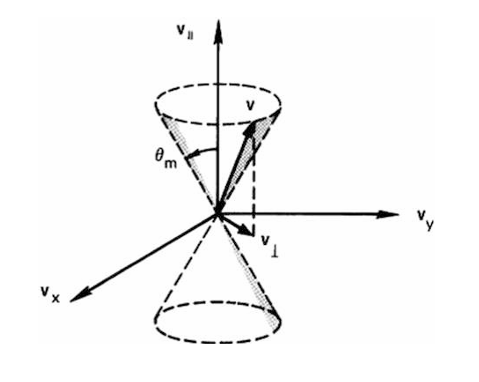
\includegraphics[width=0.7\linewidth]{loss_cone.png}
  \caption{ロスコーン}
  \label{loss_cone}
\end{figure}









\section{流体としてのプラズマ}
\subsection{導入}
プラズマでは、前章の状況よりもはるかに複雑である。電場と磁場は与えられたものではなく、電荷自体の位置と運動によって決定される。すなわち、粒子が軌道に沿って移動する際に場を生成し、かつ場が粒子をそれらの正確な軌道上を移動させるようにする。このような自己整合的な問題を解かなければならない。さらにこれは時間変動する状況下で行わなければならない。

典型的なプラズマ密度は1$\si{\metre^2}$あたり$10^{18}$個のイオン・電子対である。これらの粒子がそれぞれ複雑な軌跡を描き、それらすべてを追跡する必要があるならば、プラズマの挙動を予測することは絶望的である。幸いなことに、実際の実験で観測されるプラズマ現象の大部分(おそらく80\%ほど)は、かなり大雑把なモデルで説明できる。
このモデルは流体力学で用いられるもので、個々の粒子の同一性は無視され、流体要素の動きのみが考慮される。衝突が一般的に稀なプラズマにこのようなモデルが適用できるのは驚くべきことだと思うが、これの理由があることが後でわかるだろう。
この章ではプラズマの流体理論から得られる事実を述べる。より洗練されたプラズマの運動論は7章で扱う。

一部のプラズマ問題では、流体理論も運動論もプラズマの挙動を記述するには不十分である。その場合、個々の軌跡を追跡するという煩雑なプロセスをコンピュータによって計算するしかない。理論と実験の間の隔たりを埋める上で、コンピュータシミュレーションは重要な役割を果たしている。

\subsection{運動の流体方程式}
\subsubsection{対流微分}

粒子1個の運動方程式は、
\begin{equation}
  m\frac{d\bm{v}}{dt} = q(\bm{E}+\bm{v}\times \bm{B}) \label{normal.eq}
\end{equation}
衝突も熱運動もないと仮定すると流体要素内の全粒子は共に運動し、要素内の粒子の平均速度$\bm{u}$は個々の粒子速度$\bm{v}$と同一となる。流体方程式は\eqref{normal.eq}式に密度nを乗じるだけで得られ、

\begin{equation}
  mn\frac{d\bm{u}}{dt} = qn(\bm{E}+\bm{u}\times \bm{B}) \label{fluid_eq}
\end{equation}
となる。しかし、この方程式は使うのには不便である。というのも、\eqref{fluid_eq}式は粒子とともに移動する座標系で成り立っている。我々が欲しいのは空間に固定された座標での流体方程式である。
ある点$\bm{G}$におけるこれらの座標系の変換は、

\begin{equation}
  \frac{d\bm{G}}{dt} = \frac{\partial \bm{G}}{\partial t} + (\bm{u}\cdot \nabla)\bm{G}
\end{equation}
で表される。これの導出は\url{https://eman-physics.net/fluid/lagrange_derivative.html}を見てほしい。この関係式は対流微分もしくはラグランジュ微分と呼ばれる。
左辺は「流体要素(粒子)と一緒に動く立場」で見たときの時間変化であり、右辺第1項は「固定した位置」での時間の変化である。右辺第2項は移動による変化の寄与であり、対流項と呼ばれる。













\section{結論}
LaTeXを使えば、美しい日本語の文書を作成することができます。ぜひ活用してみてください。




\begin{thebibliography}{99}
\bibitem{a} Francis F. Chen, Introduction to Plasma Physics and Controlled Fusion, Springer; Softcover reprint of the original 3rd ed., 2019\par
\url{http://library.unisel.edu.my/equip-unisel/custom/ebook_catalog/2016BookIntroductionToPlasmaPhysicsAndcompressed.pdf}
\bibitem{b} 宮本健郎, プラズマ物理の基礎, 朝倉書店 , 2014\par
\url{https://op.lib.kobe-u.ac.jp/opac/opac_details/?reqCode=fromlist&lang=0&amode=11&bibid=2002133568&opkey=B175679900718865&start=1&totalnum=4&listnum=1&place=&list_disp=20&list_sort=0&cmode=0&chk_st=0&check=0000}
\bibitem{c} EMANの物理学\par
\url{https://eman-physics.net/electromag/plasma.html}
\end{thebibliography}





\end{document}